\begin{frame}
    \frametitle{Visualizzare ed Elaborare documenti XML}
    \addtocounter{nframe}{1}
    
        \textit{tutti i nomi di elementi TEI devono essere preceduti dal
        prefisso \textbf{tei:}}

    \begin{center}
        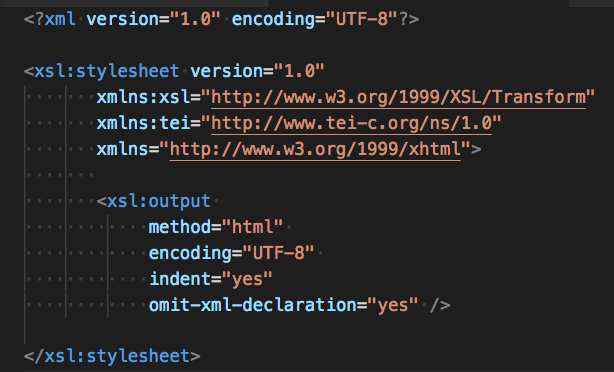
\includegraphics[width=.8\textwidth]{imgs/EsempioCommentato1.png}
    \end{center}

\end{frame}


\begin{frame}
    \frametitle{Visualizzare ed Elaborare documenti XML}
    \addtocounter{nframe}{1}
    
        \textit{creare lo “scheletro” del documento finale, nel nostro caso un HTML}

    \begin{center}
        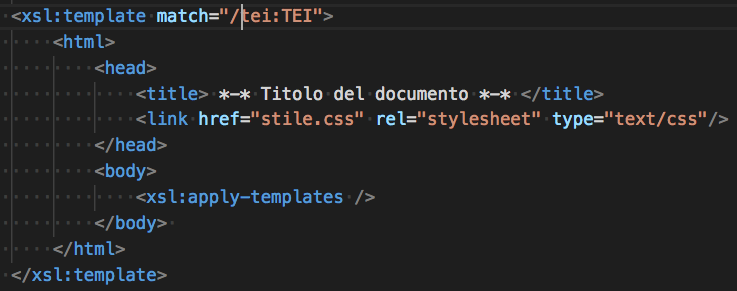
\includegraphics[width=.8\textwidth]{imgs/EsempioCommentato2.png}
    \end{center}

\end{frame}

\begin{frame}
    \frametitle{Visualizzare ed Elaborare documenti XML}
    \addtocounter{nframe}{1}
    
        \textit{definire ad esempio una regola per l’intestazione TEI (\texttt{<teiHeader>})}

    \begin{center}
        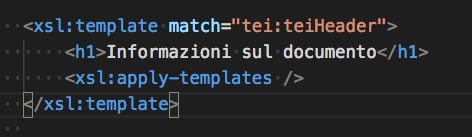
\includegraphics[width=.8\textwidth]{imgs/EsempioCommentato3.png}
    \end{center}

\end{frame}


\begin{frame}
    \frametitle{Visualizzare ed Elaborare documenti XML}
    \addtocounter{nframe}{1}
    
        \textit{Componenti dell'elemento \textbf{tei:text}}

    \begin{center}
        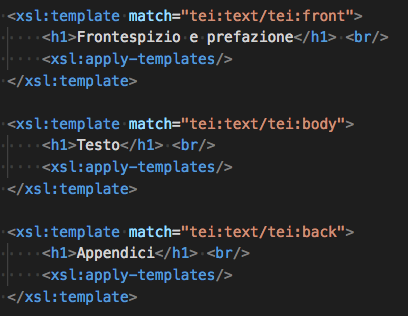
\includegraphics[width=.8\textwidth]{imgs/EsempioCommentato4.png}
    \end{center}

\end{frame}

\begin{frame}
    \frametitle{Visualizzare ed Elaborare documenti XML}
    \addtocounter{nframe}{1}
    
        \textit{Divisioni del testo}

    \begin{center}
        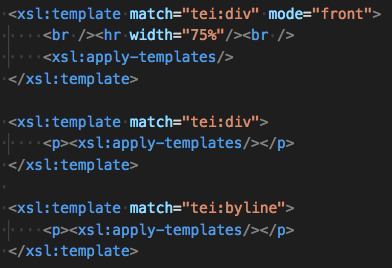
\includegraphics[width=.8\textwidth]{imgs/EsempioCommentato5.png}
    \end{center}

\end{frame}


\begin{frame}
    \frametitle{Visualizzare ed Elaborare documenti XML}
    \addtocounter{nframe}{1}
    
        \textit{Per la poesia}

    \begin{center}
        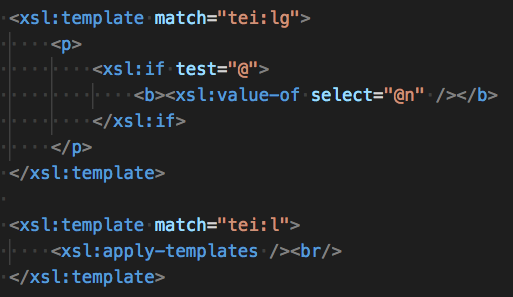
\includegraphics[width=.8\textwidth]{imgs/EsempioCommentato6.png}
    \end{center}

\end{frame}


\begin{frame}
    \frametitle{Visualizzare ed Elaborare documenti XML}
    \addtocounter{nframe}{1}
    
        \textit{Elementi Phrase-Level}

    \begin{center}
        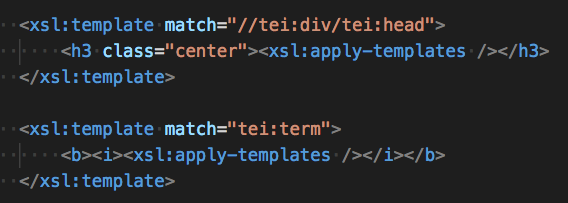
\includegraphics[width=.8\textwidth]{imgs/EsempioCommentato7.png}
    \end{center}

\end{frame}


\begin{frame}
    \frametitle{Visualizzare ed Elaborare documenti XML}
    \addtocounter{nframe}{1}
    
        \textit{Interventi Editoriali}

    \begin{center}
        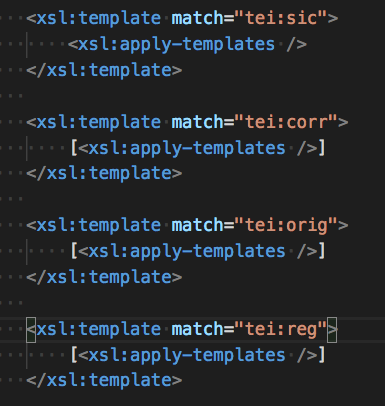
\includegraphics[width=.8\textwidth]{imgs/EsempioCommentato8.png}
    \end{center}

\end{frame}

\begin{frame}
    \frametitle{Visualizzare ed Elaborare documenti XML}
    \addtocounter{nframe}{1}
    
        \textit{Altri elementi}

    \begin{center}
        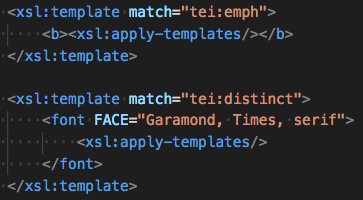
\includegraphics[width=.8\textwidth]{imgs/EsempioCommentato9.png}
    \end{center}

\end{frame}

\begin{frame}
    \frametitle{Visualizzare ed Elaborare documenti XML}
    \addtocounter{nframe}{1}
    
        \textit{Elemento \texttt{<hi>} distinto in base all'attributo \texttt{@rend}}

    \begin{center}
        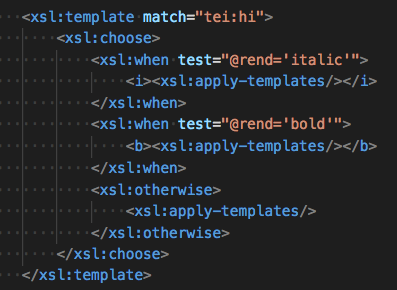
\includegraphics[width=.8\textwidth]{imgs/EsempioCommentato10.png}
    \end{center}

\end{frame}

\begin{frame}
    \frametitle{Visualizzare ed Elaborare documenti XML}
    \addtocounter{nframe}{1}
    
        \textit{Elementi vuoti e milestone}

    \begin{center}
        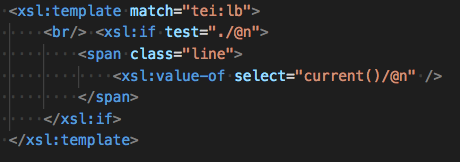
\includegraphics[width=.8\textwidth]{imgs/EsempioCommentato11.png}
    \end{center}

\end{frame}




